% Created by tikzDevice version 0.12 on 2019-08-21 20:00:52
% !TEX encoding = UTF-8 Unicode
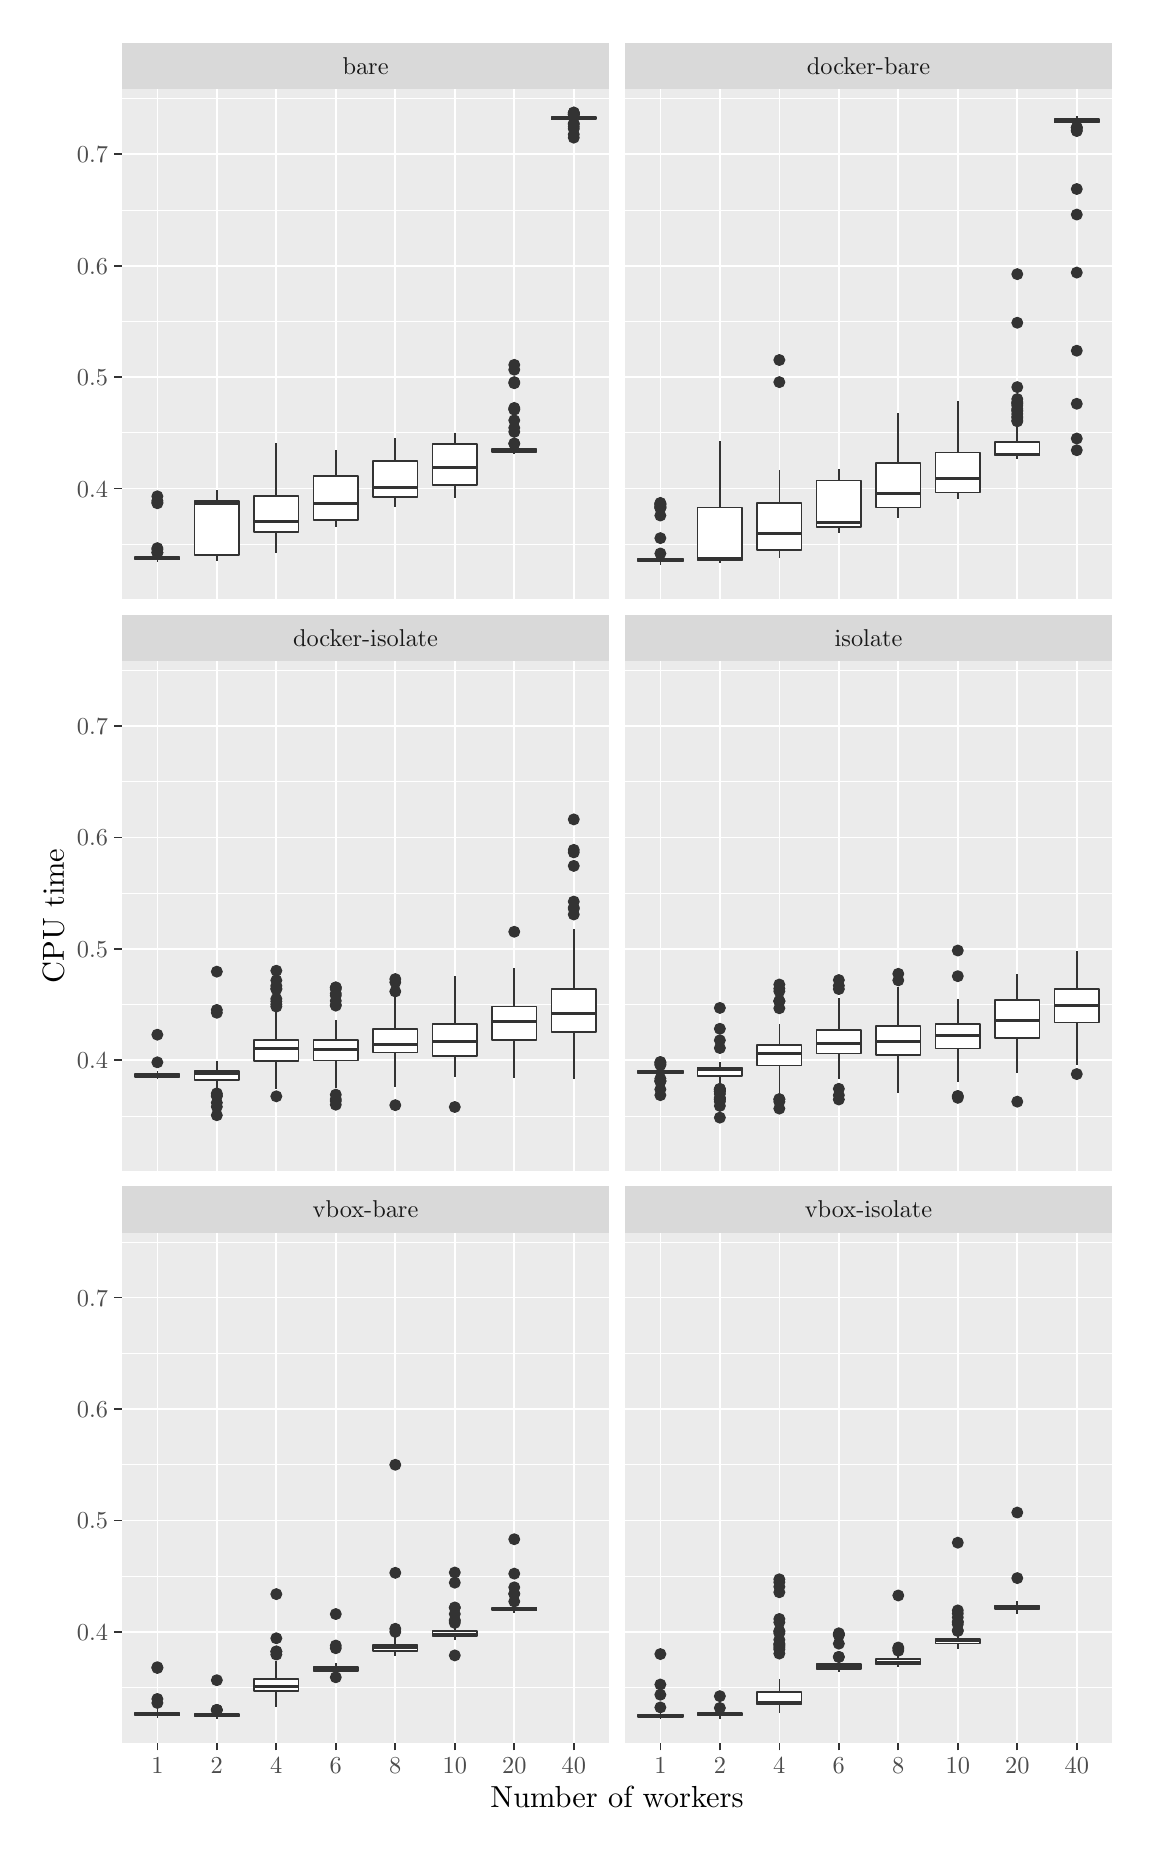
\begin{tikzpicture}[x=1pt,y=1pt]
\definecolor{fillColor}{RGB}{255,255,255}
\path[use as bounding box,fill=fillColor,fill opacity=0.00] (0,0) rectangle (397.48,650.43);
\begin{scope}
\path[clip] (  0.00,  0.00) rectangle (397.48,650.43);
\definecolor{drawColor}{RGB}{255,255,255}
\definecolor{fillColor}{RGB}{255,255,255}

\path[draw=drawColor,line width= 0.6pt,line join=round,line cap=round,fill=fillColor] (  0.00, -0.00) rectangle (397.48,650.43);
\end{scope}
\begin{scope}
\path[clip] ( 33.96,443.86) rectangle (210.22,628.13);
\definecolor{fillColor}{gray}{0.92}

\path[fill=fillColor] ( 33.96,443.86) rectangle (210.22,628.13);
\definecolor{drawColor}{RGB}{255,255,255}

\path[draw=drawColor,line width= 0.3pt,line join=round] ( 33.96,463.72) --
	(210.22,463.72);

\path[draw=drawColor,line width= 0.3pt,line join=round] ( 33.96,503.99) --
	(210.22,503.99);

\path[draw=drawColor,line width= 0.3pt,line join=round] ( 33.96,544.25) --
	(210.22,544.25);

\path[draw=drawColor,line width= 0.3pt,line join=round] ( 33.96,584.52) --
	(210.22,584.52);

\path[draw=drawColor,line width= 0.3pt,line join=round] ( 33.96,624.79) --
	(210.22,624.79);

\path[draw=drawColor,line width= 0.6pt,line join=round] ( 33.96,483.85) --
	(210.22,483.85);

\path[draw=drawColor,line width= 0.6pt,line join=round] ( 33.96,524.12) --
	(210.22,524.12);

\path[draw=drawColor,line width= 0.6pt,line join=round] ( 33.96,564.39) --
	(210.22,564.39);

\path[draw=drawColor,line width= 0.6pt,line join=round] ( 33.96,604.66) --
	(210.22,604.66);

\path[draw=drawColor,line width= 0.6pt,line join=round] ( 46.86,443.86) --
	( 46.86,628.13);

\path[draw=drawColor,line width= 0.6pt,line join=round] ( 68.35,443.86) --
	( 68.35,628.13);

\path[draw=drawColor,line width= 0.6pt,line join=round] ( 89.85,443.86) --
	( 89.85,628.13);

\path[draw=drawColor,line width= 0.6pt,line join=round] (111.34,443.86) --
	(111.34,628.13);

\path[draw=drawColor,line width= 0.6pt,line join=round] (132.84,443.86) --
	(132.84,628.13);

\path[draw=drawColor,line width= 0.6pt,line join=round] (154.34,443.86) --
	(154.34,628.13);

\path[draw=drawColor,line width= 0.6pt,line join=round] (175.83,443.86) --
	(175.83,628.13);

\path[draw=drawColor,line width= 0.6pt,line join=round] (197.33,443.86) --
	(197.33,628.13);
\definecolor{drawColor}{gray}{0.20}
\definecolor{fillColor}{gray}{0.20}

\path[draw=drawColor,line width= 0.4pt,line join=round,line cap=round,fill=fillColor] ( 46.86,481.09) circle (  1.96);

\path[draw=drawColor,line width= 0.4pt,line join=round,line cap=round,fill=fillColor] ( 46.86,460.71) circle (  1.96);

\path[draw=drawColor,line width= 0.4pt,line join=round,line cap=round,fill=fillColor] ( 46.86,462.35) circle (  1.96);

\path[draw=drawColor,line width= 0.4pt,line join=round,line cap=round,fill=fillColor] ( 46.86,478.56) circle (  1.96);

\path[draw=drawColor,line width= 0.4pt,line join=round,line cap=round,fill=fillColor] ( 46.86,478.90) circle (  1.96);

\path[draw=drawColor,line width= 0.4pt,line join=round,line cap=round,fill=fillColor] ( 46.86,461.80) circle (  1.96);

\path[draw=drawColor,line width= 0.4pt,line join=round,line cap=round,fill=fillColor] ( 46.86,460.78) circle (  1.96);

\path[draw=drawColor,line width= 0.4pt,line join=round,line cap=round,fill=fillColor] ( 46.86,479.50) circle (  1.96);

\path[draw=drawColor,line width= 0.6pt,line join=round] ( 46.86,459.20) -- ( 46.86,460.52);

\path[draw=drawColor,line width= 0.6pt,line join=round] ( 46.86,458.27) -- ( 46.86,457.51);
\definecolor{fillColor}{RGB}{255,255,255}

\path[draw=drawColor,line width= 0.6pt,line join=round,line cap=round,fill=fillColor] ( 38.80,459.20) --
	( 38.80,458.27) --
	( 54.92,458.27) --
	( 54.92,459.20) --
	( 38.80,459.20) --
	cycle;

\path[draw=drawColor,line width= 1.1pt,line join=round] ( 38.80,458.63) -- ( 54.92,458.63);

\path[draw=drawColor,line width= 0.6pt,line join=round] ( 68.35,479.43) -- ( 68.35,483.21);

\path[draw=drawColor,line width= 0.6pt,line join=round] ( 68.35,459.86) -- ( 68.35,457.70);

\path[draw=drawColor,line width= 0.6pt,line join=round,line cap=round,fill=fillColor] ( 60.29,479.43) --
	( 60.29,459.86) --
	( 76.41,459.86) --
	( 76.41,479.43) --
	( 60.29,479.43) --
	cycle;

\path[draw=drawColor,line width= 1.1pt,line join=round] ( 60.29,478.46) -- ( 76.41,478.46);

\path[draw=drawColor,line width= 0.6pt,line join=round] ( 89.85,481.18) -- ( 89.85,500.17);

\path[draw=drawColor,line width= 0.6pt,line join=round] ( 89.85,468.15) -- ( 89.85,460.56);

\path[draw=drawColor,line width= 0.6pt,line join=round,line cap=round,fill=fillColor] ( 81.79,481.18) --
	( 81.79,468.15) --
	( 97.91,468.15) --
	( 97.91,481.18) --
	( 81.79,481.18) --
	cycle;

\path[draw=drawColor,line width= 1.1pt,line join=round] ( 81.79,471.98) -- ( 97.91,471.98);

\path[draw=drawColor,line width= 0.6pt,line join=round] (111.34,488.37) -- (111.34,497.66);

\path[draw=drawColor,line width= 0.6pt,line join=round] (111.34,472.56) -- (111.34,469.90);

\path[draw=drawColor,line width= 0.6pt,line join=round,line cap=round,fill=fillColor] (103.28,488.37) --
	(103.28,472.56) --
	(119.41,472.56) --
	(119.41,488.37) --
	(103.28,488.37) --
	cycle;

\path[draw=drawColor,line width= 1.1pt,line join=round] (103.28,478.53) -- (119.41,478.53);

\path[draw=drawColor,line width= 0.6pt,line join=round] (132.84,493.81) -- (132.84,502.21);

\path[draw=drawColor,line width= 0.6pt,line join=round] (132.84,480.83) -- (132.84,477.24);

\path[draw=drawColor,line width= 0.6pt,line join=round,line cap=round,fill=fillColor] (124.78,493.81) --
	(124.78,480.83) --
	(140.90,480.83) --
	(140.90,493.81) --
	(124.78,493.81) --
	cycle;

\path[draw=drawColor,line width= 1.1pt,line join=round] (124.78,484.15) -- (140.90,484.15);

\path[draw=drawColor,line width= 0.6pt,line join=round] (154.34,500.01) -- (154.34,504.01);

\path[draw=drawColor,line width= 0.6pt,line join=round] (154.34,485.12) -- (154.34,480.63);

\path[draw=drawColor,line width= 0.6pt,line join=round,line cap=round,fill=fillColor] (146.27,500.01) --
	(146.27,485.12) --
	(162.40,485.12) --
	(162.40,500.01) --
	(146.27,500.01) --
	cycle;

\path[draw=drawColor,line width= 1.1pt,line join=round] (146.27,491.38) -- (162.40,491.38);
\definecolor{fillColor}{gray}{0.20}

\path[draw=drawColor,line width= 0.4pt,line join=round,line cap=round,fill=fillColor] (175.83,513.02) circle (  1.96);

\path[draw=drawColor,line width= 0.4pt,line join=round,line cap=round,fill=fillColor] (175.83,528.58) circle (  1.96);

\path[draw=drawColor,line width= 0.4pt,line join=round,line cap=round,fill=fillColor] (175.83,500.13) circle (  1.96);

\path[draw=drawColor,line width= 0.4pt,line join=round,line cap=round,fill=fillColor] (175.83,500.15) circle (  1.96);

\path[draw=drawColor,line width= 0.4pt,line join=round,line cap=round,fill=fillColor] (175.83,526.83) circle (  1.96);

\path[draw=drawColor,line width= 0.4pt,line join=round,line cap=round,fill=fillColor] (175.83,522.34) circle (  1.96);

\path[draw=drawColor,line width= 0.4pt,line join=round,line cap=round,fill=fillColor] (175.83,512.57) circle (  1.96);

\path[draw=drawColor,line width= 0.4pt,line join=round,line cap=round,fill=fillColor] (175.83,504.37) circle (  1.96);

\path[draw=drawColor,line width= 0.4pt,line join=round,line cap=round,fill=fillColor] (175.83,512.40) circle (  1.96);

\path[draw=drawColor,line width= 0.4pt,line join=round,line cap=round,fill=fillColor] (175.83,521.94) circle (  1.96);

\path[draw=drawColor,line width= 0.4pt,line join=round,line cap=round,fill=fillColor] (175.83,505.83) circle (  1.96);

\path[draw=drawColor,line width= 0.4pt,line join=round,line cap=round,fill=fillColor] (175.83,508.53) circle (  1.96);

\path[draw=drawColor,line width= 0.6pt,line join=round] (175.83,498.26) -- (175.83,499.68);

\path[draw=drawColor,line width= 0.6pt,line join=round] (175.83,497.18) -- (175.83,496.28);
\definecolor{fillColor}{RGB}{255,255,255}

\path[draw=drawColor,line width= 0.6pt,line join=round,line cap=round,fill=fillColor] (167.77,498.26) --
	(167.77,497.18) --
	(183.89,497.18) --
	(183.89,498.26) --
	(167.77,498.26) --
	cycle;

\path[draw=drawColor,line width= 1.1pt,line join=round] (167.77,497.63) -- (183.89,497.63);
\definecolor{fillColor}{gray}{0.20}

\path[draw=drawColor,line width= 0.4pt,line join=round,line cap=round,fill=fillColor] (197.33,610.68) circle (  1.96);

\path[draw=drawColor,line width= 0.4pt,line join=round,line cap=round,fill=fillColor] (197.33,614.66) circle (  1.96);

\path[draw=drawColor,line width= 0.4pt,line join=round,line cap=round,fill=fillColor] (197.33,619.01) circle (  1.96);

\path[draw=drawColor,line width= 0.4pt,line join=round,line cap=round,fill=fillColor] (197.33,615.52) circle (  1.96);

\path[draw=drawColor,line width= 0.4pt,line join=round,line cap=round,fill=fillColor] (197.33,619.44) circle (  1.96);

\path[draw=drawColor,line width= 0.4pt,line join=round,line cap=round,fill=fillColor] (197.33,613.88) circle (  1.96);

\path[draw=drawColor,line width= 0.4pt,line join=round,line cap=round,fill=fillColor] (197.33,611.85) circle (  1.96);

\path[draw=drawColor,line width= 0.4pt,line join=round,line cap=round,fill=fillColor] (197.33,619.05) circle (  1.96);

\path[draw=drawColor,line width= 0.4pt,line join=round,line cap=round,fill=fillColor] (197.33,619.00) circle (  1.96);

\path[draw=drawColor,line width= 0.4pt,line join=round,line cap=round,fill=fillColor] (197.33,615.86) circle (  1.96);

\path[draw=drawColor,line width= 0.4pt,line join=round,line cap=round,fill=fillColor] (197.33,619.75) circle (  1.96);

\path[draw=drawColor,line width= 0.4pt,line join=round,line cap=round,fill=fillColor] (197.33,619.73) circle (  1.96);

\path[draw=drawColor,line width= 0.6pt,line join=round] (197.33,618.04) -- (197.33,618.96);

\path[draw=drawColor,line width= 0.6pt,line join=round] (197.33,617.41) -- (197.33,616.69);
\definecolor{fillColor}{RGB}{255,255,255}

\path[draw=drawColor,line width= 0.6pt,line join=round,line cap=round,fill=fillColor] (189.27,618.04) --
	(189.27,617.41) --
	(205.39,617.41) --
	(205.39,618.04) --
	(189.27,618.04) --
	cycle;

\path[draw=drawColor,line width= 1.1pt,line join=round] (189.27,617.63) -- (205.39,617.63);
\end{scope}
\begin{scope}
\path[clip] ( 33.96,237.29) rectangle (210.22,421.56);
\definecolor{fillColor}{gray}{0.92}

\path[fill=fillColor] ( 33.96,237.29) rectangle (210.22,421.56);
\definecolor{drawColor}{RGB}{255,255,255}

\path[draw=drawColor,line width= 0.3pt,line join=round] ( 33.96,257.15) --
	(210.22,257.15);

\path[draw=drawColor,line width= 0.3pt,line join=round] ( 33.96,297.42) --
	(210.22,297.42);

\path[draw=drawColor,line width= 0.3pt,line join=round] ( 33.96,337.69) --
	(210.22,337.69);

\path[draw=drawColor,line width= 0.3pt,line join=round] ( 33.96,377.95) --
	(210.22,377.95);

\path[draw=drawColor,line width= 0.3pt,line join=round] ( 33.96,418.22) --
	(210.22,418.22);

\path[draw=drawColor,line width= 0.6pt,line join=round] ( 33.96,277.28) --
	(210.22,277.28);

\path[draw=drawColor,line width= 0.6pt,line join=round] ( 33.96,317.55) --
	(210.22,317.55);

\path[draw=drawColor,line width= 0.6pt,line join=round] ( 33.96,357.82) --
	(210.22,357.82);

\path[draw=drawColor,line width= 0.6pt,line join=round] ( 33.96,398.09) --
	(210.22,398.09);

\path[draw=drawColor,line width= 0.6pt,line join=round] ( 46.86,237.29) --
	( 46.86,421.56);

\path[draw=drawColor,line width= 0.6pt,line join=round] ( 68.35,237.29) --
	( 68.35,421.56);

\path[draw=drawColor,line width= 0.6pt,line join=round] ( 89.85,237.29) --
	( 89.85,421.56);

\path[draw=drawColor,line width= 0.6pt,line join=round] (111.34,237.29) --
	(111.34,421.56);

\path[draw=drawColor,line width= 0.6pt,line join=round] (132.84,237.29) --
	(132.84,421.56);

\path[draw=drawColor,line width= 0.6pt,line join=round] (154.34,237.29) --
	(154.34,421.56);

\path[draw=drawColor,line width= 0.6pt,line join=round] (175.83,237.29) --
	(175.83,421.56);

\path[draw=drawColor,line width= 0.6pt,line join=round] (197.33,237.29) --
	(197.33,421.56);
\definecolor{drawColor}{gray}{0.20}
\definecolor{fillColor}{gray}{0.20}

\path[draw=drawColor,line width= 0.4pt,line join=round,line cap=round,fill=fillColor] ( 46.86,286.54) circle (  1.96);

\path[draw=drawColor,line width= 0.4pt,line join=round,line cap=round,fill=fillColor] ( 46.86,276.56) circle (  1.96);

\path[draw=drawColor,line width= 0.6pt,line join=round] ( 46.86,272.33) -- ( 46.86,273.46);

\path[draw=drawColor,line width= 0.6pt,line join=round] ( 46.86,271.31) -- ( 46.86,270.57);
\definecolor{fillColor}{RGB}{255,255,255}

\path[draw=drawColor,line width= 0.6pt,line join=round,line cap=round,fill=fillColor] ( 38.80,272.33) --
	( 38.80,271.31) --
	( 54.92,271.31) --
	( 54.92,272.33) --
	( 38.80,272.33) --
	cycle;

\path[draw=drawColor,line width= 1.1pt,line join=round] ( 38.80,271.77) -- ( 54.92,271.77);
\definecolor{fillColor}{gray}{0.20}

\path[draw=drawColor,line width= 0.4pt,line join=round,line cap=round,fill=fillColor] ( 68.35,294.46) circle (  1.96);

\path[draw=drawColor,line width= 0.4pt,line join=round,line cap=round,fill=fillColor] ( 68.35,265.33) circle (  1.96);

\path[draw=drawColor,line width= 0.4pt,line join=round,line cap=round,fill=fillColor] ( 68.35,260.50) circle (  1.96);

\path[draw=drawColor,line width= 0.4pt,line join=round,line cap=round,fill=fillColor] ( 68.35,309.32) circle (  1.96);

\path[draw=drawColor,line width= 0.4pt,line join=round,line cap=round,fill=fillColor] ( 68.35,261.96) circle (  1.96);

\path[draw=drawColor,line width= 0.4pt,line join=round,line cap=round,fill=fillColor] ( 68.35,264.27) circle (  1.96);

\path[draw=drawColor,line width= 0.4pt,line join=round,line cap=round,fill=fillColor] ( 68.35,295.49) circle (  1.96);

\path[draw=drawColor,line width= 0.4pt,line join=round,line cap=round,fill=fillColor] ( 68.35,257.43) circle (  1.96);

\path[draw=drawColor,line width= 0.4pt,line join=round,line cap=round,fill=fillColor] ( 68.35,264.73) circle (  1.96);

\path[draw=drawColor,line width= 0.6pt,line join=round] ( 68.35,273.31) -- ( 68.35,276.90);

\path[draw=drawColor,line width= 0.6pt,line join=round] ( 68.35,270.20) -- ( 68.35,265.82);
\definecolor{fillColor}{RGB}{255,255,255}

\path[draw=drawColor,line width= 0.6pt,line join=round,line cap=round,fill=fillColor] ( 60.29,273.31) --
	( 60.29,270.20) --
	( 76.41,270.20) --
	( 76.41,273.31) --
	( 60.29,273.31) --
	cycle;

\path[draw=drawColor,line width= 1.1pt,line join=round] ( 60.29,272.43) -- ( 76.41,272.43);
\definecolor{fillColor}{gray}{0.20}

\path[draw=drawColor,line width= 0.4pt,line join=round,line cap=round,fill=fillColor] ( 89.85,304.21) circle (  1.96);

\path[draw=drawColor,line width= 0.4pt,line join=round,line cap=round,fill=fillColor] ( 89.85,302.95) circle (  1.96);

\path[draw=drawColor,line width= 0.4pt,line join=round,line cap=round,fill=fillColor] ( 89.85,306.18) circle (  1.96);

\path[draw=drawColor,line width= 0.4pt,line join=round,line cap=round,fill=fillColor] ( 89.85,309.66) circle (  1.96);

\path[draw=drawColor,line width= 0.4pt,line join=round,line cap=round,fill=fillColor] ( 89.85,303.27) circle (  1.96);

\path[draw=drawColor,line width= 0.4pt,line join=round,line cap=round,fill=fillColor] ( 89.85,296.70) circle (  1.96);

\path[draw=drawColor,line width= 0.4pt,line join=round,line cap=round,fill=fillColor] ( 89.85,264.27) circle (  1.96);

\path[draw=drawColor,line width= 0.4pt,line join=round,line cap=round,fill=fillColor] ( 89.85,299.51) circle (  1.96);

\path[draw=drawColor,line width= 0.4pt,line join=round,line cap=round,fill=fillColor] ( 89.85,297.52) circle (  1.96);

\path[draw=drawColor,line width= 0.4pt,line join=round,line cap=round,fill=fillColor] ( 89.85,298.58) circle (  1.96);

\path[draw=drawColor,line width= 0.6pt,line join=round] ( 89.85,284.72) -- ( 89.85,294.76);

\path[draw=drawColor,line width= 0.6pt,line join=round] ( 89.85,277.03) -- ( 89.85,266.96);
\definecolor{fillColor}{RGB}{255,255,255}

\path[draw=drawColor,line width= 0.6pt,line join=round,line cap=round,fill=fillColor] ( 81.79,284.72) --
	( 81.79,277.03) --
	( 97.91,277.03) --
	( 97.91,284.72) --
	( 81.79,284.72) --
	cycle;

\path[draw=drawColor,line width= 1.1pt,line join=round] ( 81.79,281.42) -- ( 97.91,281.42);
\definecolor{fillColor}{gray}{0.20}

\path[draw=drawColor,line width= 0.4pt,line join=round,line cap=round,fill=fillColor] (111.34,301.42) circle (  1.96);

\path[draw=drawColor,line width= 0.4pt,line join=round,line cap=round,fill=fillColor] (111.34,303.63) circle (  1.96);

\path[draw=drawColor,line width= 0.4pt,line join=round,line cap=round,fill=fillColor] (111.34,298.79) circle (  1.96);

\path[draw=drawColor,line width= 0.4pt,line join=round,line cap=round,fill=fillColor] (111.34,261.24) circle (  1.96);

\path[draw=drawColor,line width= 0.4pt,line join=round,line cap=round,fill=fillColor] (111.34,297.34) circle (  1.96);

\path[draw=drawColor,line width= 0.4pt,line join=round,line cap=round,fill=fillColor] (111.34,300.67) circle (  1.96);

\path[draw=drawColor,line width= 0.4pt,line join=round,line cap=round,fill=fillColor] (111.34,303.61) circle (  1.96);

\path[draw=drawColor,line width= 0.4pt,line join=round,line cap=round,fill=fillColor] (111.34,262.57) circle (  1.96);

\path[draw=drawColor,line width= 0.4pt,line join=round,line cap=round,fill=fillColor] (111.34,297.04) circle (  1.96);

\path[draw=drawColor,line width= 0.4pt,line join=round,line cap=round,fill=fillColor] (111.34,264.87) circle (  1.96);

\path[draw=drawColor,line width= 0.4pt,line join=round,line cap=round,fill=fillColor] (111.34,303.00) circle (  1.96);

\path[draw=drawColor,line width= 0.4pt,line join=round,line cap=round,fill=fillColor] (111.34,263.27) circle (  1.96);

\path[draw=drawColor,line width= 0.6pt,line join=round] (111.34,284.52) -- (111.34,291.73);

\path[draw=drawColor,line width= 0.6pt,line join=round] (111.34,277.16) -- (111.34,267.15);
\definecolor{fillColor}{RGB}{255,255,255}

\path[draw=drawColor,line width= 0.6pt,line join=round,line cap=round,fill=fillColor] (103.28,284.52) --
	(103.28,277.16) --
	(119.41,277.16) --
	(119.41,284.52) --
	(103.28,284.52) --
	cycle;

\path[draw=drawColor,line width= 1.1pt,line join=round] (103.28,281.14) -- (119.41,281.14);
\definecolor{fillColor}{gray}{0.20}

\path[draw=drawColor,line width= 0.4pt,line join=round,line cap=round,fill=fillColor] (132.84,261.07) circle (  1.96);

\path[draw=drawColor,line width= 0.4pt,line join=round,line cap=round,fill=fillColor] (132.84,305.45) circle (  1.96);

\path[draw=drawColor,line width= 0.4pt,line join=round,line cap=round,fill=fillColor] (132.84,302.16) circle (  1.96);

\path[draw=drawColor,line width= 0.4pt,line join=round,line cap=round,fill=fillColor] (132.84,306.64) circle (  1.96);

\path[draw=drawColor,line width= 0.6pt,line join=round] (132.84,288.66) -- (132.84,300.92);

\path[draw=drawColor,line width= 0.6pt,line join=round] (132.84,280.12) -- (132.84,267.58);
\definecolor{fillColor}{RGB}{255,255,255}

\path[draw=drawColor,line width= 0.6pt,line join=round,line cap=round,fill=fillColor] (124.78,288.66) --
	(124.78,280.12) --
	(140.90,280.12) --
	(140.90,288.66) --
	(124.78,288.66) --
	cycle;

\path[draw=drawColor,line width= 1.1pt,line join=round] (124.78,282.86) -- (140.90,282.86);
\definecolor{fillColor}{gray}{0.20}

\path[draw=drawColor,line width= 0.4pt,line join=round,line cap=round,fill=fillColor] (154.34,260.41) circle (  1.96);

\path[draw=drawColor,line width= 0.6pt,line join=round] (154.34,290.50) -- (154.34,307.67);

\path[draw=drawColor,line width= 0.6pt,line join=round] (154.34,278.78) -- (154.34,271.23);
\definecolor{fillColor}{RGB}{255,255,255}

\path[draw=drawColor,line width= 0.6pt,line join=round,line cap=round,fill=fillColor] (146.27,290.50) --
	(146.27,278.78) --
	(162.40,278.78) --
	(162.40,290.50) --
	(146.27,290.50) --
	cycle;

\path[draw=drawColor,line width= 1.1pt,line join=round] (146.27,284.22) -- (162.40,284.22);
\definecolor{fillColor}{gray}{0.20}

\path[draw=drawColor,line width= 0.4pt,line join=round,line cap=round,fill=fillColor] (175.83,323.73) circle (  1.96);

\path[draw=drawColor,line width= 0.6pt,line join=round] (175.83,296.77) -- (175.83,310.75);

\path[draw=drawColor,line width= 0.6pt,line join=round] (175.83,284.70) -- (175.83,271.06);
\definecolor{fillColor}{RGB}{255,255,255}

\path[draw=drawColor,line width= 0.6pt,line join=round,line cap=round,fill=fillColor] (167.77,296.77) --
	(167.77,284.70) --
	(183.89,284.70) --
	(183.89,296.77) --
	(167.77,296.77) --
	cycle;

\path[draw=drawColor,line width= 1.1pt,line join=round] (167.77,291.14) -- (183.89,291.14);
\definecolor{fillColor}{gray}{0.20}

\path[draw=drawColor,line width= 0.4pt,line join=round,line cap=round,fill=fillColor] (197.33,332.01) circle (  1.96);

\path[draw=drawColor,line width= 0.4pt,line join=round,line cap=round,fill=fillColor] (197.33,364.33) circle (  1.96);

\path[draw=drawColor,line width= 0.4pt,line join=round,line cap=round,fill=fillColor] (197.33,334.64) circle (  1.96);

\path[draw=drawColor,line width= 0.4pt,line join=round,line cap=round,fill=fillColor] (197.33,352.41) circle (  1.96);

\path[draw=drawColor,line width= 0.4pt,line join=round,line cap=round,fill=fillColor] (197.33,347.53) circle (  1.96);

\path[draw=drawColor,line width= 0.4pt,line join=round,line cap=round,fill=fillColor] (197.33,329.98) circle (  1.96);

\path[draw=drawColor,line width= 0.4pt,line join=round,line cap=round,fill=fillColor] (197.33,353.33) circle (  1.96);

\path[draw=drawColor,line width= 0.4pt,line join=round,line cap=round,fill=fillColor] (197.33,332.48) circle (  1.96);

\path[draw=drawColor,line width= 0.6pt,line join=round] (197.33,303.14) -- (197.33,324.83);

\path[draw=drawColor,line width= 0.6pt,line join=round] (197.33,287.52) -- (197.33,270.58);
\definecolor{fillColor}{RGB}{255,255,255}

\path[draw=drawColor,line width= 0.6pt,line join=round,line cap=round,fill=fillColor] (189.27,303.14) --
	(189.27,287.52) --
	(205.39,287.52) --
	(205.39,303.14) --
	(189.27,303.14) --
	cycle;

\path[draw=drawColor,line width= 1.1pt,line join=round] (189.27,294.30) -- (205.39,294.30);
\end{scope}
\begin{scope}
\path[clip] ( 33.96, 30.72) rectangle (210.22,214.99);
\definecolor{fillColor}{gray}{0.92}

\path[fill=fillColor] ( 33.96, 30.72) rectangle (210.22,214.99);
\definecolor{drawColor}{RGB}{255,255,255}

\path[draw=drawColor,line width= 0.3pt,line join=round] ( 33.96, 50.58) --
	(210.22, 50.58);

\path[draw=drawColor,line width= 0.3pt,line join=round] ( 33.96, 90.85) --
	(210.22, 90.85);

\path[draw=drawColor,line width= 0.3pt,line join=round] ( 33.96,131.12) --
	(210.22,131.12);

\path[draw=drawColor,line width= 0.3pt,line join=round] ( 33.96,171.39) --
	(210.22,171.39);

\path[draw=drawColor,line width= 0.3pt,line join=round] ( 33.96,211.65) --
	(210.22,211.65);

\path[draw=drawColor,line width= 0.6pt,line join=round] ( 33.96, 70.72) --
	(210.22, 70.72);

\path[draw=drawColor,line width= 0.6pt,line join=round] ( 33.96,110.98) --
	(210.22,110.98);

\path[draw=drawColor,line width= 0.6pt,line join=round] ( 33.96,151.25) --
	(210.22,151.25);

\path[draw=drawColor,line width= 0.6pt,line join=round] ( 33.96,191.52) --
	(210.22,191.52);

\path[draw=drawColor,line width= 0.6pt,line join=round] ( 46.86, 30.72) --
	( 46.86,214.99);

\path[draw=drawColor,line width= 0.6pt,line join=round] ( 68.35, 30.72) --
	( 68.35,214.99);

\path[draw=drawColor,line width= 0.6pt,line join=round] ( 89.85, 30.72) --
	( 89.85,214.99);

\path[draw=drawColor,line width= 0.6pt,line join=round] (111.34, 30.72) --
	(111.34,214.99);

\path[draw=drawColor,line width= 0.6pt,line join=round] (132.84, 30.72) --
	(132.84,214.99);

\path[draw=drawColor,line width= 0.6pt,line join=round] (154.34, 30.72) --
	(154.34,214.99);

\path[draw=drawColor,line width= 0.6pt,line join=round] (175.83, 30.72) --
	(175.83,214.99);

\path[draw=drawColor,line width= 0.6pt,line join=round] (197.33, 30.72) --
	(197.33,214.99);
\definecolor{drawColor}{gray}{0.20}
\definecolor{fillColor}{gray}{0.20}

\path[draw=drawColor,line width= 0.4pt,line join=round,line cap=round,fill=fillColor] ( 46.86, 57.99) circle (  1.96);

\path[draw=drawColor,line width= 0.4pt,line join=round,line cap=round,fill=fillColor] ( 46.86, 45.08) circle (  1.96);

\path[draw=drawColor,line width= 0.4pt,line join=round,line cap=round,fill=fillColor] ( 46.86, 57.70) circle (  1.96);

\path[draw=drawColor,line width= 0.4pt,line join=round,line cap=round,fill=fillColor] ( 46.86, 46.51) circle (  1.96);

\path[draw=drawColor,line width= 0.6pt,line join=round] ( 46.86, 41.66) -- ( 46.86, 42.76);

\path[draw=drawColor,line width= 0.6pt,line join=round] ( 46.86, 40.56) -- ( 46.86, 39.67);
\definecolor{fillColor}{RGB}{255,255,255}

\path[draw=drawColor,line width= 0.6pt,line join=round,line cap=round,fill=fillColor] ( 38.80, 41.66) --
	( 38.80, 40.56) --
	( 54.92, 40.56) --
	( 54.92, 41.66) --
	( 38.80, 41.66) --
	cycle;

\path[draw=drawColor,line width= 1.1pt,line join=round] ( 38.80, 40.92) -- ( 54.92, 40.92);
\definecolor{fillColor}{gray}{0.20}

\path[draw=drawColor,line width= 0.4pt,line join=round,line cap=round,fill=fillColor] ( 68.35, 53.29) circle (  1.96);

\path[draw=drawColor,line width= 0.4pt,line join=round,line cap=round,fill=fillColor] ( 68.35, 42.56) circle (  1.96);

\path[draw=drawColor,line width= 0.4pt,line join=round,line cap=round,fill=fillColor] ( 68.35, 42.51) circle (  1.96);

\path[draw=drawColor,line width= 0.4pt,line join=round,line cap=round,fill=fillColor] ( 68.35, 42.52) circle (  1.96);

\path[draw=drawColor,line width= 0.6pt,line join=round] ( 68.35, 40.99) -- ( 68.35, 42.12);

\path[draw=drawColor,line width= 0.6pt,line join=round] ( 68.35, 40.13) -- ( 68.35, 39.13);
\definecolor{fillColor}{RGB}{255,255,255}

\path[draw=drawColor,line width= 0.6pt,line join=round,line cap=round,fill=fillColor] ( 60.29, 40.99) --
	( 60.29, 40.13) --
	( 76.41, 40.13) --
	( 76.41, 40.99) --
	( 60.29, 40.99) --
	cycle;

\path[draw=drawColor,line width= 1.1pt,line join=round] ( 60.29, 40.48) -- ( 76.41, 40.48);
\definecolor{fillColor}{gray}{0.20}

\path[draw=drawColor,line width= 0.4pt,line join=round,line cap=round,fill=fillColor] ( 89.85, 62.56) circle (  1.96);

\path[draw=drawColor,line width= 0.4pt,line join=round,line cap=round,fill=fillColor] ( 89.85, 84.39) circle (  1.96);

\path[draw=drawColor,line width= 0.4pt,line join=round,line cap=round,fill=fillColor] ( 89.85, 63.72) circle (  1.96);

\path[draw=drawColor,line width= 0.4pt,line join=round,line cap=round,fill=fillColor] ( 89.85, 63.59) circle (  1.96);

\path[draw=drawColor,line width= 0.4pt,line join=round,line cap=round,fill=fillColor] ( 89.85, 68.44) circle (  1.96);

\path[draw=drawColor,line width= 0.6pt,line join=round] ( 89.85, 53.83) -- ( 89.85, 60.12);

\path[draw=drawColor,line width= 0.6pt,line join=round] ( 89.85, 49.38) -- ( 89.85, 43.59);
\definecolor{fillColor}{RGB}{255,255,255}

\path[draw=drawColor,line width= 0.6pt,line join=round,line cap=round,fill=fillColor] ( 81.79, 53.83) --
	( 81.79, 49.38) --
	( 97.91, 49.38) --
	( 97.91, 53.83) --
	( 81.79, 53.83) --
	cycle;

\path[draw=drawColor,line width= 1.1pt,line join=round] ( 81.79, 50.84) -- ( 97.91, 50.84);
\definecolor{fillColor}{gray}{0.20}

\path[draw=drawColor,line width= 0.4pt,line join=round,line cap=round,fill=fillColor] (111.34, 77.19) circle (  1.96);

\path[draw=drawColor,line width= 0.4pt,line join=round,line cap=round,fill=fillColor] (111.34, 54.34) circle (  1.96);

\path[draw=drawColor,line width= 0.4pt,line join=round,line cap=round,fill=fillColor] (111.34, 64.84) circle (  1.96);

\path[draw=drawColor,line width= 0.4pt,line join=round,line cap=round,fill=fillColor] (111.34, 65.81) circle (  1.96);

\path[draw=drawColor,line width= 0.6pt,line join=round] (111.34, 58.13) -- (111.34, 59.64);

\path[draw=drawColor,line width= 0.6pt,line join=round] (111.34, 56.66) -- (111.34, 55.29);
\definecolor{fillColor}{RGB}{255,255,255}

\path[draw=drawColor,line width= 0.6pt,line join=round,line cap=round,fill=fillColor] (103.28, 58.13) --
	(103.28, 56.66) --
	(119.41, 56.66) --
	(119.41, 58.13) --
	(103.28, 58.13) --
	cycle;

\path[draw=drawColor,line width= 1.1pt,line join=round] (103.28, 57.44) -- (119.41, 57.44);
\definecolor{fillColor}{gray}{0.20}

\path[draw=drawColor,line width= 0.4pt,line join=round,line cap=round,fill=fillColor] (132.84,131.13) circle (  1.96);

\path[draw=drawColor,line width= 0.4pt,line join=round,line cap=round,fill=fillColor] (132.84, 70.75) circle (  1.96);

\path[draw=drawColor,line width= 0.4pt,line join=round,line cap=round,fill=fillColor] (132.84, 71.87) circle (  1.96);

\path[draw=drawColor,line width= 0.4pt,line join=round,line cap=round,fill=fillColor] (132.84, 92.09) circle (  1.96);

\path[draw=drawColor,line width= 0.6pt,line join=round] (132.84, 66.02) -- (132.84, 69.19);

\path[draw=drawColor,line width= 0.6pt,line join=round] (132.84, 63.79) -- (132.84, 61.93);
\definecolor{fillColor}{RGB}{255,255,255}

\path[draw=drawColor,line width= 0.6pt,line join=round,line cap=round,fill=fillColor] (124.78, 66.02) --
	(124.78, 63.79) --
	(140.90, 63.79) --
	(140.90, 66.02) --
	(124.78, 66.02) --
	cycle;

\path[draw=drawColor,line width= 1.1pt,line join=round] (124.78, 65.00) -- (140.90, 65.00);
\definecolor{fillColor}{gray}{0.20}

\path[draw=drawColor,line width= 0.4pt,line join=round,line cap=round,fill=fillColor] (154.34, 79.57) circle (  1.96);

\path[draw=drawColor,line width= 0.4pt,line join=round,line cap=round,fill=fillColor] (154.34, 77.21) circle (  1.96);

\path[draw=drawColor,line width= 0.4pt,line join=round,line cap=round,fill=fillColor] (154.34, 75.03) circle (  1.96);

\path[draw=drawColor,line width= 0.4pt,line join=round,line cap=round,fill=fillColor] (154.34, 73.98) circle (  1.96);

\path[draw=drawColor,line width= 0.4pt,line join=round,line cap=round,fill=fillColor] (154.34, 74.67) circle (  1.96);

\path[draw=drawColor,line width= 0.4pt,line join=round,line cap=round,fill=fillColor] (154.34, 92.20) circle (  1.96);

\path[draw=drawColor,line width= 0.4pt,line join=round,line cap=round,fill=fillColor] (154.34, 88.53) circle (  1.96);

\path[draw=drawColor,line width= 0.4pt,line join=round,line cap=round,fill=fillColor] (154.34, 62.25) circle (  1.96);

\path[draw=drawColor,line width= 0.4pt,line join=round,line cap=round,fill=fillColor] (154.34, 79.47) circle (  1.96);

\path[draw=drawColor,line width= 0.6pt,line join=round] (154.34, 71.07) -- (154.34, 73.09);

\path[draw=drawColor,line width= 0.6pt,line join=round] (154.34, 69.28) -- (154.34, 67.70);
\definecolor{fillColor}{RGB}{255,255,255}

\path[draw=drawColor,line width= 0.6pt,line join=round,line cap=round,fill=fillColor] (146.27, 71.07) --
	(146.27, 69.28) --
	(162.40, 69.28) --
	(162.40, 71.07) --
	(146.27, 71.07) --
	cycle;

\path[draw=drawColor,line width= 1.1pt,line join=round] (146.27, 69.85) -- (162.40, 69.85);
\definecolor{fillColor}{gray}{0.20}

\path[draw=drawColor,line width= 0.4pt,line join=round,line cap=round,fill=fillColor] (175.83, 86.84) circle (  1.96);

\path[draw=drawColor,line width= 0.4pt,line join=round,line cap=round,fill=fillColor] (175.83, 84.54) circle (  1.96);

\path[draw=drawColor,line width= 0.4pt,line join=round,line cap=round,fill=fillColor] (175.83, 84.46) circle (  1.96);

\path[draw=drawColor,line width= 0.4pt,line join=round,line cap=round,fill=fillColor] (175.83,104.23) circle (  1.96);

\path[draw=drawColor,line width= 0.4pt,line join=round,line cap=round,fill=fillColor] (175.83, 91.79) circle (  1.96);

\path[draw=drawColor,line width= 0.4pt,line join=round,line cap=round,fill=fillColor] (175.83, 81.74) circle (  1.96);

\path[draw=drawColor,line width= 0.6pt,line join=round] (175.83, 79.49) -- (175.83, 80.45);

\path[draw=drawColor,line width= 0.6pt,line join=round] (175.83, 78.54) -- (175.83, 77.57);
\definecolor{fillColor}{RGB}{255,255,255}

\path[draw=drawColor,line width= 0.6pt,line join=round,line cap=round,fill=fillColor] (167.77, 79.49) --
	(167.77, 78.54) --
	(183.89, 78.54) --
	(183.89, 79.49) --
	(167.77, 79.49) --
	cycle;

\path[draw=drawColor,line width= 1.1pt,line join=round] (167.77, 79.01) -- (183.89, 79.01);
\end{scope}
\begin{scope}
\path[clip] (215.72,443.86) rectangle (391.98,628.13);
\definecolor{fillColor}{gray}{0.92}

\path[fill=fillColor] (215.72,443.86) rectangle (391.98,628.13);
\definecolor{drawColor}{RGB}{255,255,255}

\path[draw=drawColor,line width= 0.3pt,line join=round] (215.72,463.72) --
	(391.98,463.72);

\path[draw=drawColor,line width= 0.3pt,line join=round] (215.72,503.99) --
	(391.98,503.99);

\path[draw=drawColor,line width= 0.3pt,line join=round] (215.72,544.25) --
	(391.98,544.25);

\path[draw=drawColor,line width= 0.3pt,line join=round] (215.72,584.52) --
	(391.98,584.52);

\path[draw=drawColor,line width= 0.3pt,line join=round] (215.72,624.79) --
	(391.98,624.79);

\path[draw=drawColor,line width= 0.6pt,line join=round] (215.72,483.85) --
	(391.98,483.85);

\path[draw=drawColor,line width= 0.6pt,line join=round] (215.72,524.12) --
	(391.98,524.12);

\path[draw=drawColor,line width= 0.6pt,line join=round] (215.72,564.39) --
	(391.98,564.39);

\path[draw=drawColor,line width= 0.6pt,line join=round] (215.72,604.66) --
	(391.98,604.66);

\path[draw=drawColor,line width= 0.6pt,line join=round] (228.62,443.86) --
	(228.62,628.13);

\path[draw=drawColor,line width= 0.6pt,line join=round] (250.12,443.86) --
	(250.12,628.13);

\path[draw=drawColor,line width= 0.6pt,line join=round] (271.61,443.86) --
	(271.61,628.13);

\path[draw=drawColor,line width= 0.6pt,line join=round] (293.11,443.86) --
	(293.11,628.13);

\path[draw=drawColor,line width= 0.6pt,line join=round] (314.60,443.86) --
	(314.60,628.13);

\path[draw=drawColor,line width= 0.6pt,line join=round] (336.10,443.86) --
	(336.10,628.13);

\path[draw=drawColor,line width= 0.6pt,line join=round] (357.59,443.86) --
	(357.59,628.13);

\path[draw=drawColor,line width= 0.6pt,line join=round] (379.09,443.86) --
	(379.09,628.13);
\definecolor{drawColor}{gray}{0.20}
\definecolor{fillColor}{gray}{0.20}

\path[draw=drawColor,line width= 0.4pt,line join=round,line cap=round,fill=fillColor] (228.62,474.14) circle (  1.96);

\path[draw=drawColor,line width= 0.4pt,line join=round,line cap=round,fill=fillColor] (228.62,478.40) circle (  1.96);

\path[draw=drawColor,line width= 0.4pt,line join=round,line cap=round,fill=fillColor] (228.62,478.19) circle (  1.96);

\path[draw=drawColor,line width= 0.4pt,line join=round,line cap=round,fill=fillColor] (228.62,477.42) circle (  1.96);

\path[draw=drawColor,line width= 0.4pt,line join=round,line cap=round,fill=fillColor] (228.62,477.93) circle (  1.96);

\path[draw=drawColor,line width= 0.4pt,line join=round,line cap=round,fill=fillColor] (228.62,460.42) circle (  1.96);

\path[draw=drawColor,line width= 0.4pt,line join=round,line cap=round,fill=fillColor] (228.62,477.18) circle (  1.96);

\path[draw=drawColor,line width= 0.4pt,line join=round,line cap=round,fill=fillColor] (228.62,476.83) circle (  1.96);

\path[draw=drawColor,line width= 0.4pt,line join=round,line cap=round,fill=fillColor] (228.62,476.86) circle (  1.96);

\path[draw=drawColor,line width= 0.4pt,line join=round,line cap=round,fill=fillColor] (228.62,478.70) circle (  1.96);

\path[draw=drawColor,line width= 0.4pt,line join=round,line cap=round,fill=fillColor] (228.62,465.97) circle (  1.96);

\path[draw=drawColor,line width= 0.6pt,line join=round] (228.62,458.66) -- (228.62,460.39);

\path[draw=drawColor,line width= 0.6pt,line join=round] (228.62,457.49) -- (228.62,456.42);
\definecolor{fillColor}{RGB}{255,255,255}

\path[draw=drawColor,line width= 0.6pt,line join=round,line cap=round,fill=fillColor] (220.56,458.66) --
	(220.56,457.49) --
	(236.68,457.49) --
	(236.68,458.66) --
	(220.56,458.66) --
	cycle;

\path[draw=drawColor,line width= 1.1pt,line join=round] (220.56,458.01) -- (236.68,458.01);

\path[draw=drawColor,line width= 0.6pt,line join=round] (250.12,477.03) -- (250.12,501.03);

\path[draw=drawColor,line width= 0.6pt,line join=round] (250.12,457.91) -- (250.12,456.93);

\path[draw=drawColor,line width= 0.6pt,line join=round,line cap=round,fill=fillColor] (242.06,477.03) --
	(242.06,457.91) --
	(258.18,457.91) --
	(258.18,477.03) --
	(242.06,477.03) --
	cycle;

\path[draw=drawColor,line width= 1.1pt,line join=round] (242.06,458.67) -- (258.18,458.67);
\definecolor{fillColor}{gray}{0.20}

\path[draw=drawColor,line width= 0.4pt,line join=round,line cap=round,fill=fillColor] (271.61,522.34) circle (  1.96);

\path[draw=drawColor,line width= 0.4pt,line join=round,line cap=round,fill=fillColor] (271.61,530.33) circle (  1.96);

\path[draw=drawColor,line width= 0.6pt,line join=round] (271.61,478.65) -- (271.61,490.65);

\path[draw=drawColor,line width= 0.6pt,line join=round] (271.61,461.77) -- (271.61,458.61);
\definecolor{fillColor}{RGB}{255,255,255}

\path[draw=drawColor,line width= 0.6pt,line join=round,line cap=round,fill=fillColor] (263.55,478.65) --
	(263.55,461.77) --
	(279.67,461.77) --
	(279.67,478.65) --
	(263.55,478.65) --
	cycle;

\path[draw=drawColor,line width= 1.1pt,line join=round] (263.55,467.62) -- (279.67,467.62);

\path[draw=drawColor,line width= 0.6pt,line join=round] (293.11,486.83) -- (293.11,491.13);

\path[draw=drawColor,line width= 0.6pt,line join=round] (293.11,470.00) -- (293.11,467.68);

\path[draw=drawColor,line width= 0.6pt,line join=round,line cap=round,fill=fillColor] (285.05,486.83) --
	(285.05,470.00) --
	(301.17,470.00) --
	(301.17,486.83) --
	(285.05,486.83) --
	cycle;

\path[draw=drawColor,line width= 1.1pt,line join=round] (285.05,471.73) -- (301.17,471.73);

\path[draw=drawColor,line width= 0.6pt,line join=round] (314.60,493.04) -- (314.60,511.27);

\path[draw=drawColor,line width= 0.6pt,line join=round] (314.60,477.08) -- (314.60,473.10);

\path[draw=drawColor,line width= 0.6pt,line join=round,line cap=round,fill=fillColor] (306.54,493.04) --
	(306.54,477.08) --
	(322.66,477.08) --
	(322.66,493.04) --
	(306.54,493.04) --
	cycle;

\path[draw=drawColor,line width= 1.1pt,line join=round] (306.54,481.98) -- (322.66,481.98);

\path[draw=drawColor,line width= 0.6pt,line join=round] (336.10,496.93) -- (336.10,515.65);

\path[draw=drawColor,line width= 0.6pt,line join=round] (336.10,482.48) -- (336.10,480.00);

\path[draw=drawColor,line width= 0.6pt,line join=round,line cap=round,fill=fillColor] (328.04,496.93) --
	(328.04,482.48) --
	(344.16,482.48) --
	(344.16,496.93) --
	(328.04,496.93) --
	cycle;

\path[draw=drawColor,line width= 1.1pt,line join=round] (328.04,487.46) -- (344.16,487.46);
\definecolor{fillColor}{gray}{0.20}

\path[draw=drawColor,line width= 0.4pt,line join=round,line cap=round,fill=fillColor] (357.59,514.80) circle (  1.96);

\path[draw=drawColor,line width= 0.4pt,line join=round,line cap=round,fill=fillColor] (357.59,509.44) circle (  1.96);

\path[draw=drawColor,line width= 0.4pt,line join=round,line cap=round,fill=fillColor] (357.59,520.54) circle (  1.96);

\path[draw=drawColor,line width= 0.4pt,line join=round,line cap=round,fill=fillColor] (357.59,510.85) circle (  1.96);

\path[draw=drawColor,line width= 0.4pt,line join=round,line cap=round,fill=fillColor] (357.59,508.49) circle (  1.96);

\path[draw=drawColor,line width= 0.4pt,line join=round,line cap=round,fill=fillColor] (357.59,511.85) circle (  1.96);

\path[draw=drawColor,line width= 0.4pt,line join=round,line cap=round,fill=fillColor] (357.59,512.16) circle (  1.96);

\path[draw=drawColor,line width= 0.4pt,line join=round,line cap=round,fill=fillColor] (357.59,509.92) circle (  1.96);

\path[draw=drawColor,line width= 0.4pt,line join=round,line cap=round,fill=fillColor] (357.59,514.52) circle (  1.96);

\path[draw=drawColor,line width= 0.4pt,line join=round,line cap=round,fill=fillColor] (357.59,516.22) circle (  1.96);

\path[draw=drawColor,line width= 0.4pt,line join=round,line cap=round,fill=fillColor] (357.59,561.36) circle (  1.96);

\path[draw=drawColor,line width= 0.4pt,line join=round,line cap=round,fill=fillColor] (357.59,515.18) circle (  1.96);

\path[draw=drawColor,line width= 0.4pt,line join=round,line cap=round,fill=fillColor] (357.59,508.18) circle (  1.96);

\path[draw=drawColor,line width= 0.4pt,line join=round,line cap=round,fill=fillColor] (357.59,543.80) circle (  1.96);

\path[draw=drawColor,line width= 0.4pt,line join=round,line cap=round,fill=fillColor] (357.59,513.87) circle (  1.96);

\path[draw=drawColor,line width= 0.4pt,line join=round,line cap=round,fill=fillColor] (357.59,512.73) circle (  1.96);

\path[draw=drawColor,line width= 0.6pt,line join=round] (357.59,500.70) -- (357.59,507.18);

\path[draw=drawColor,line width= 0.6pt,line join=round] (357.59,495.79) -- (357.59,494.53);
\definecolor{fillColor}{RGB}{255,255,255}

\path[draw=drawColor,line width= 0.6pt,line join=round,line cap=round,fill=fillColor] (349.53,500.70) --
	(349.53,495.79) --
	(365.65,495.79) --
	(365.65,500.70) --
	(349.53,500.70) --
	cycle;

\path[draw=drawColor,line width= 1.1pt,line join=round] (349.53,496.33) -- (365.65,496.33);
\definecolor{fillColor}{gray}{0.20}

\path[draw=drawColor,line width= 0.4pt,line join=round,line cap=round,fill=fillColor] (379.09,501.96) circle (  1.96);

\path[draw=drawColor,line width= 0.4pt,line join=round,line cap=round,fill=fillColor] (379.09,514.52) circle (  1.96);

\path[draw=drawColor,line width= 0.4pt,line join=round,line cap=round,fill=fillColor] (379.09,497.73) circle (  1.96);

\path[draw=drawColor,line width= 0.4pt,line join=round,line cap=round,fill=fillColor] (379.09,533.70) circle (  1.96);

\path[draw=drawColor,line width= 0.4pt,line join=round,line cap=round,fill=fillColor] (379.09,582.89) circle (  1.96);

\path[draw=drawColor,line width= 0.4pt,line join=round,line cap=round,fill=fillColor] (379.09,561.93) circle (  1.96);

\path[draw=drawColor,line width= 0.4pt,line join=round,line cap=round,fill=fillColor] (379.09,592.12) circle (  1.96);

\path[draw=drawColor,line width= 0.4pt,line join=round,line cap=round,fill=fillColor] (379.09,613.37) circle (  1.96);

\path[draw=drawColor,line width= 0.4pt,line join=round,line cap=round,fill=fillColor] (379.09,614.29) circle (  1.96);

\path[draw=drawColor,line width= 0.4pt,line join=round,line cap=round,fill=fillColor] (379.09,614.21) circle (  1.96);

\path[draw=drawColor,line width= 0.4pt,line join=round,line cap=round,fill=fillColor] (379.09,613.06) circle (  1.96);

\path[draw=drawColor,line width= 0.4pt,line join=round,line cap=round,fill=fillColor] (379.09,614.43) circle (  1.96);

\path[draw=drawColor,line width= 0.6pt,line join=round] (379.09,617.32) -- (379.09,618.58);

\path[draw=drawColor,line width= 0.6pt,line join=round] (379.09,616.19) -- (379.09,614.56);
\definecolor{fillColor}{RGB}{255,255,255}

\path[draw=drawColor,line width= 0.6pt,line join=round,line cap=round,fill=fillColor] (371.03,617.32) --
	(371.03,616.19) --
	(387.15,616.19) --
	(387.15,617.32) --
	(371.03,617.32) --
	cycle;

\path[draw=drawColor,line width= 1.1pt,line join=round] (371.03,616.66) -- (387.15,616.66);
\end{scope}
\begin{scope}
\path[clip] (215.72,237.29) rectangle (391.98,421.56);
\definecolor{fillColor}{gray}{0.92}

\path[fill=fillColor] (215.72,237.29) rectangle (391.98,421.56);
\definecolor{drawColor}{RGB}{255,255,255}

\path[draw=drawColor,line width= 0.3pt,line join=round] (215.72,257.15) --
	(391.98,257.15);

\path[draw=drawColor,line width= 0.3pt,line join=round] (215.72,297.42) --
	(391.98,297.42);

\path[draw=drawColor,line width= 0.3pt,line join=round] (215.72,337.69) --
	(391.98,337.69);

\path[draw=drawColor,line width= 0.3pt,line join=round] (215.72,377.95) --
	(391.98,377.95);

\path[draw=drawColor,line width= 0.3pt,line join=round] (215.72,418.22) --
	(391.98,418.22);

\path[draw=drawColor,line width= 0.6pt,line join=round] (215.72,277.28) --
	(391.98,277.28);

\path[draw=drawColor,line width= 0.6pt,line join=round] (215.72,317.55) --
	(391.98,317.55);

\path[draw=drawColor,line width= 0.6pt,line join=round] (215.72,357.82) --
	(391.98,357.82);

\path[draw=drawColor,line width= 0.6pt,line join=round] (215.72,398.09) --
	(391.98,398.09);

\path[draw=drawColor,line width= 0.6pt,line join=round] (228.62,237.29) --
	(228.62,421.56);

\path[draw=drawColor,line width= 0.6pt,line join=round] (250.12,237.29) --
	(250.12,421.56);

\path[draw=drawColor,line width= 0.6pt,line join=round] (271.61,237.29) --
	(271.61,421.56);

\path[draw=drawColor,line width= 0.6pt,line join=round] (293.11,237.29) --
	(293.11,421.56);

\path[draw=drawColor,line width= 0.6pt,line join=round] (314.60,237.29) --
	(314.60,421.56);

\path[draw=drawColor,line width= 0.6pt,line join=round] (336.10,237.29) --
	(336.10,421.56);

\path[draw=drawColor,line width= 0.6pt,line join=round] (357.59,237.29) --
	(357.59,421.56);

\path[draw=drawColor,line width= 0.6pt,line join=round] (379.09,237.29) --
	(379.09,421.56);
\definecolor{drawColor}{gray}{0.20}
\definecolor{fillColor}{gray}{0.20}

\path[draw=drawColor,line width= 0.4pt,line join=round,line cap=round,fill=fillColor] (228.62,275.56) circle (  1.96);

\path[draw=drawColor,line width= 0.4pt,line join=round,line cap=round,fill=fillColor] (228.62,266.78) circle (  1.96);

\path[draw=drawColor,line width= 0.4pt,line join=round,line cap=round,fill=fillColor] (228.62,275.94) circle (  1.96);

\path[draw=drawColor,line width= 0.4pt,line join=round,line cap=round,fill=fillColor] (228.62,276.69) circle (  1.96);

\path[draw=drawColor,line width= 0.4pt,line join=round,line cap=round,fill=fillColor] (228.62,269.92) circle (  1.96);

\path[draw=drawColor,line width= 0.4pt,line join=round,line cap=round,fill=fillColor] (228.62,276.46) circle (  1.96);

\path[draw=drawColor,line width= 0.4pt,line join=round,line cap=round,fill=fillColor] (228.62,269.58) circle (  1.96);

\path[draw=drawColor,line width= 0.4pt,line join=round,line cap=round,fill=fillColor] (228.62,270.70) circle (  1.96);

\path[draw=drawColor,line width= 0.4pt,line join=round,line cap=round,fill=fillColor] (228.62,264.69) circle (  1.96);

\path[draw=drawColor,line width= 0.4pt,line join=round,line cap=round,fill=fillColor] (228.62,269.82) circle (  1.96);

\path[draw=drawColor,line width= 0.6pt,line join=round] (228.62,273.61) -- (228.62,275.15);

\path[draw=drawColor,line width= 0.6pt,line join=round] (228.62,272.48) -- (228.62,270.98);
\definecolor{fillColor}{RGB}{255,255,255}

\path[draw=drawColor,line width= 0.6pt,line join=round,line cap=round,fill=fillColor] (220.56,273.61) --
	(220.56,272.48) --
	(236.68,272.48) --
	(236.68,273.61) --
	(220.56,273.61) --
	cycle;

\path[draw=drawColor,line width= 1.1pt,line join=round] (220.56,273.26) -- (236.68,273.26);
\definecolor{fillColor}{gray}{0.20}

\path[draw=drawColor,line width= 0.4pt,line join=round,line cap=round,fill=fillColor] (250.12,266.05) circle (  1.96);

\path[draw=drawColor,line width= 0.4pt,line join=round,line cap=round,fill=fillColor] (250.12,256.57) circle (  1.96);

\path[draw=drawColor,line width= 0.4pt,line join=round,line cap=round,fill=fillColor] (250.12,263.28) circle (  1.96);

\path[draw=drawColor,line width= 0.4pt,line join=round,line cap=round,fill=fillColor] (250.12,284.52) circle (  1.96);

\path[draw=drawColor,line width= 0.4pt,line join=round,line cap=round,fill=fillColor] (250.12,263.20) circle (  1.96);

\path[draw=drawColor,line width= 0.4pt,line join=round,line cap=round,fill=fillColor] (250.12,260.81) circle (  1.96);

\path[draw=drawColor,line width= 0.4pt,line join=round,line cap=round,fill=fillColor] (250.12,296.21) circle (  1.96);

\path[draw=drawColor,line width= 0.4pt,line join=round,line cap=round,fill=fillColor] (250.12,288.68) circle (  1.96);

\path[draw=drawColor,line width= 0.4pt,line join=round,line cap=round,fill=fillColor] (250.12,266.76) circle (  1.96);

\path[draw=drawColor,line width= 0.4pt,line join=round,line cap=round,fill=fillColor] (250.12,265.14) circle (  1.96);

\path[draw=drawColor,line width= 0.4pt,line join=round,line cap=round,fill=fillColor] (250.12,262.35) circle (  1.96);

\path[draw=drawColor,line width= 0.4pt,line join=round,line cap=round,fill=fillColor] (250.12,263.78) circle (  1.96);

\path[draw=drawColor,line width= 0.4pt,line join=round,line cap=round,fill=fillColor] (250.12,266.05) circle (  1.96);

\path[draw=drawColor,line width= 0.4pt,line join=round,line cap=round,fill=fillColor] (250.12,281.72) circle (  1.96);

\path[draw=drawColor,line width= 0.4pt,line join=round,line cap=round,fill=fillColor] (250.12,263.22) circle (  1.96);

\path[draw=drawColor,line width= 0.4pt,line join=round,line cap=round,fill=fillColor] (250.12,266.98) circle (  1.96);

\path[draw=drawColor,line width= 0.4pt,line join=round,line cap=round,fill=fillColor] (250.12,266.59) circle (  1.96);

\path[draw=drawColor,line width= 0.4pt,line join=round,line cap=round,fill=fillColor] (250.12,266.83) circle (  1.96);

\path[draw=drawColor,line width= 0.6pt,line join=round] (250.12,274.64) -- (250.12,276.71);

\path[draw=drawColor,line width= 0.6pt,line join=round] (250.12,271.63) -- (250.12,268.18);
\definecolor{fillColor}{RGB}{255,255,255}

\path[draw=drawColor,line width= 0.6pt,line join=round,line cap=round,fill=fillColor] (242.06,274.64) --
	(242.06,271.63) --
	(258.18,271.63) --
	(258.18,274.64) --
	(242.06,274.64) --
	cycle;

\path[draw=drawColor,line width= 1.1pt,line join=round] (242.06,273.94) -- (258.18,273.94);
\definecolor{fillColor}{gray}{0.20}

\path[draw=drawColor,line width= 0.4pt,line join=round,line cap=round,fill=fillColor] (271.61,259.84) circle (  1.96);

\path[draw=drawColor,line width= 0.4pt,line join=round,line cap=round,fill=fillColor] (271.61,263.18) circle (  1.96);

\path[draw=drawColor,line width= 0.4pt,line join=round,line cap=round,fill=fillColor] (271.61,262.31) circle (  1.96);

\path[draw=drawColor,line width= 0.4pt,line join=round,line cap=round,fill=fillColor] (271.61,303.20) circle (  1.96);

\path[draw=drawColor,line width= 0.4pt,line join=round,line cap=round,fill=fillColor] (271.61,298.66) circle (  1.96);

\path[draw=drawColor,line width= 0.4pt,line join=round,line cap=round,fill=fillColor] (271.61,298.76) circle (  1.96);

\path[draw=drawColor,line width= 0.4pt,line join=round,line cap=round,fill=fillColor] (271.61,298.59) circle (  1.96);

\path[draw=drawColor,line width= 0.4pt,line join=round,line cap=round,fill=fillColor] (271.61,296.09) circle (  1.96);

\path[draw=drawColor,line width= 0.4pt,line join=round,line cap=round,fill=fillColor] (271.61,263.26) circle (  1.96);

\path[draw=drawColor,line width= 0.4pt,line join=round,line cap=round,fill=fillColor] (271.61,302.23) circle (  1.96);

\path[draw=drawColor,line width= 0.4pt,line join=round,line cap=round,fill=fillColor] (271.61,304.67) circle (  1.96);

\path[draw=drawColor,line width= 0.6pt,line join=round] (271.61,282.84) -- (271.61,290.50);

\path[draw=drawColor,line width= 0.6pt,line join=round] (271.61,275.35) -- (271.61,264.48);
\definecolor{fillColor}{RGB}{255,255,255}

\path[draw=drawColor,line width= 0.6pt,line join=round,line cap=round,fill=fillColor] (263.55,282.84) --
	(263.55,275.35) --
	(279.67,275.35) --
	(279.67,282.84) --
	(263.55,282.84) --
	cycle;

\path[draw=drawColor,line width= 1.1pt,line join=round] (263.55,279.61) -- (279.67,279.61);
\definecolor{fillColor}{gray}{0.20}

\path[draw=drawColor,line width= 0.4pt,line join=round,line cap=round,fill=fillColor] (293.11,304.25) circle (  1.96);

\path[draw=drawColor,line width= 0.4pt,line join=round,line cap=round,fill=fillColor] (293.11,263.12) circle (  1.96);

\path[draw=drawColor,line width= 0.4pt,line join=round,line cap=round,fill=fillColor] (293.11,306.28) circle (  1.96);

\path[draw=drawColor,line width= 0.4pt,line join=round,line cap=round,fill=fillColor] (293.11,266.98) circle (  1.96);

\path[draw=drawColor,line width= 0.4pt,line join=round,line cap=round,fill=fillColor] (293.11,264.67) circle (  1.96);

\path[draw=drawColor,line width= 0.4pt,line join=round,line cap=round,fill=fillColor] (293.11,303.03) circle (  1.96);

\path[draw=drawColor,line width= 0.6pt,line join=round] (293.11,288.22) -- (293.11,299.75);

\path[draw=drawColor,line width= 0.6pt,line join=round] (293.11,279.75) -- (293.11,270.35);
\definecolor{fillColor}{RGB}{255,255,255}

\path[draw=drawColor,line width= 0.6pt,line join=round,line cap=round,fill=fillColor] (285.05,288.22) --
	(285.05,279.75) --
	(301.17,279.75) --
	(301.17,288.22) --
	(285.05,288.22) --
	cycle;

\path[draw=drawColor,line width= 1.1pt,line join=round] (285.05,283.46) -- (301.17,283.46);
\definecolor{fillColor}{gray}{0.20}

\path[draw=drawColor,line width= 0.4pt,line join=round,line cap=round,fill=fillColor] (314.60,308.54) circle (  1.96);

\path[draw=drawColor,line width= 0.4pt,line join=round,line cap=round,fill=fillColor] (314.60,306.18) circle (  1.96);

\path[draw=drawColor,line width= 0.6pt,line join=round] (314.60,289.76) -- (314.60,303.74);

\path[draw=drawColor,line width= 0.6pt,line join=round] (314.60,279.25) -- (314.60,265.44);
\definecolor{fillColor}{RGB}{255,255,255}

\path[draw=drawColor,line width= 0.6pt,line join=round,line cap=round,fill=fillColor] (306.54,289.76) --
	(306.54,279.25) --
	(322.66,279.25) --
	(322.66,289.76) --
	(306.54,289.76) --
	cycle;

\path[draw=drawColor,line width= 1.1pt,line join=round] (306.54,284.22) -- (322.66,284.22);
\definecolor{fillColor}{gray}{0.20}

\path[draw=drawColor,line width= 0.4pt,line join=round,line cap=round,fill=fillColor] (336.10,263.72) circle (  1.96);

\path[draw=drawColor,line width= 0.4pt,line join=round,line cap=round,fill=fillColor] (336.10,316.95) circle (  1.96);

\path[draw=drawColor,line width= 0.4pt,line join=round,line cap=round,fill=fillColor] (336.10,264.40) circle (  1.96);

\path[draw=drawColor,line width= 0.4pt,line join=round,line cap=round,fill=fillColor] (336.10,307.68) circle (  1.96);

\path[draw=drawColor,line width= 0.4pt,line join=round,line cap=round,fill=fillColor] (336.10,264.24) circle (  1.96);

\path[draw=drawColor,line width= 0.6pt,line join=round] (336.10,290.29) -- (336.10,299.42);

\path[draw=drawColor,line width= 0.6pt,line join=round] (336.10,281.53) -- (336.10,269.31);
\definecolor{fillColor}{RGB}{255,255,255}

\path[draw=drawColor,line width= 0.6pt,line join=round,line cap=round,fill=fillColor] (328.04,290.29) --
	(328.04,281.53) --
	(344.16,281.53) --
	(344.16,290.29) --
	(328.04,290.29) --
	cycle;

\path[draw=drawColor,line width= 1.1pt,line join=round] (328.04,286.35) -- (344.16,286.35);
\definecolor{fillColor}{gray}{0.20}

\path[draw=drawColor,line width= 0.4pt,line join=round,line cap=round,fill=fillColor] (357.59,262.34) circle (  1.96);

\path[draw=drawColor,line width= 0.6pt,line join=round] (357.59,299.17) -- (357.59,308.37);

\path[draw=drawColor,line width= 0.6pt,line join=round] (357.59,285.35) -- (357.59,272.81);
\definecolor{fillColor}{RGB}{255,255,255}

\path[draw=drawColor,line width= 0.6pt,line join=round,line cap=round,fill=fillColor] (349.53,299.17) --
	(349.53,285.35) --
	(365.65,285.35) --
	(365.65,299.17) --
	(349.53,299.17) --
	cycle;

\path[draw=drawColor,line width= 1.1pt,line join=round] (349.53,291.61) -- (365.65,291.61);
\definecolor{fillColor}{gray}{0.20}

\path[draw=drawColor,line width= 0.4pt,line join=round,line cap=round,fill=fillColor] (379.09,272.31) circle (  1.96);

\path[draw=drawColor,line width= 0.6pt,line join=round] (379.09,303.14) -- (379.09,316.90);

\path[draw=drawColor,line width= 0.6pt,line join=round] (379.09,290.93) -- (379.09,275.72);
\definecolor{fillColor}{RGB}{255,255,255}

\path[draw=drawColor,line width= 0.6pt,line join=round,line cap=round,fill=fillColor] (371.03,303.14) --
	(371.03,290.93) --
	(387.15,290.93) --
	(387.15,303.14) --
	(371.03,303.14) --
	cycle;

\path[draw=drawColor,line width= 1.1pt,line join=round] (371.03,297.14) -- (387.15,297.14);
\end{scope}
\begin{scope}
\path[clip] (215.72, 30.72) rectangle (391.98,214.99);
\definecolor{fillColor}{gray}{0.92}

\path[fill=fillColor] (215.72, 30.72) rectangle (391.98,214.99);
\definecolor{drawColor}{RGB}{255,255,255}

\path[draw=drawColor,line width= 0.3pt,line join=round] (215.72, 50.58) --
	(391.98, 50.58);

\path[draw=drawColor,line width= 0.3pt,line join=round] (215.72, 90.85) --
	(391.98, 90.85);

\path[draw=drawColor,line width= 0.3pt,line join=round] (215.72,131.12) --
	(391.98,131.12);

\path[draw=drawColor,line width= 0.3pt,line join=round] (215.72,171.39) --
	(391.98,171.39);

\path[draw=drawColor,line width= 0.3pt,line join=round] (215.72,211.65) --
	(391.98,211.65);

\path[draw=drawColor,line width= 0.6pt,line join=round] (215.72, 70.72) --
	(391.98, 70.72);

\path[draw=drawColor,line width= 0.6pt,line join=round] (215.72,110.98) --
	(391.98,110.98);

\path[draw=drawColor,line width= 0.6pt,line join=round] (215.72,151.25) --
	(391.98,151.25);

\path[draw=drawColor,line width= 0.6pt,line join=round] (215.72,191.52) --
	(391.98,191.52);

\path[draw=drawColor,line width= 0.6pt,line join=round] (228.62, 30.72) --
	(228.62,214.99);

\path[draw=drawColor,line width= 0.6pt,line join=round] (250.12, 30.72) --
	(250.12,214.99);

\path[draw=drawColor,line width= 0.6pt,line join=round] (271.61, 30.72) --
	(271.61,214.99);

\path[draw=drawColor,line width= 0.6pt,line join=round] (293.11, 30.72) --
	(293.11,214.99);

\path[draw=drawColor,line width= 0.6pt,line join=round] (314.60, 30.72) --
	(314.60,214.99);

\path[draw=drawColor,line width= 0.6pt,line join=round] (336.10, 30.72) --
	(336.10,214.99);

\path[draw=drawColor,line width= 0.6pt,line join=round] (357.59, 30.72) --
	(357.59,214.99);

\path[draw=drawColor,line width= 0.6pt,line join=round] (379.09, 30.72) --
	(379.09,214.99);
\definecolor{drawColor}{gray}{0.20}
\definecolor{fillColor}{gray}{0.20}

\path[draw=drawColor,line width= 0.4pt,line join=round,line cap=round,fill=fillColor] (228.62, 48.04) circle (  1.96);

\path[draw=drawColor,line width= 0.4pt,line join=round,line cap=round,fill=fillColor] (228.62, 43.46) circle (  1.96);

\path[draw=drawColor,line width= 0.4pt,line join=round,line cap=round,fill=fillColor] (228.62, 51.73) circle (  1.96);

\path[draw=drawColor,line width= 0.4pt,line join=round,line cap=round,fill=fillColor] (228.62, 62.73) circle (  1.96);

\path[draw=drawColor,line width= 0.6pt,line join=round] (228.62, 40.90) -- (228.62, 42.13);

\path[draw=drawColor,line width= 0.6pt,line join=round] (228.62, 39.93) -- (228.62, 39.24);
\definecolor{fillColor}{RGB}{255,255,255}

\path[draw=drawColor,line width= 0.6pt,line join=round,line cap=round,fill=fillColor] (220.56, 40.90) --
	(220.56, 39.93) --
	(236.68, 39.93) --
	(236.68, 40.90) --
	(220.56, 40.90) --
	cycle;

\path[draw=drawColor,line width= 1.1pt,line join=round] (220.56, 40.31) -- (236.68, 40.31);
\definecolor{fillColor}{gray}{0.20}

\path[draw=drawColor,line width= 0.4pt,line join=round,line cap=round,fill=fillColor] (250.12, 47.52) circle (  1.96);

\path[draw=drawColor,line width= 0.4pt,line join=round,line cap=round,fill=fillColor] (250.12, 43.26) circle (  1.96);

\path[draw=drawColor,line width= 0.6pt,line join=round] (250.12, 41.51) -- (250.12, 42.71);

\path[draw=drawColor,line width= 0.6pt,line join=round] (250.12, 40.48) -- (250.12, 39.10);
\definecolor{fillColor}{RGB}{255,255,255}

\path[draw=drawColor,line width= 0.6pt,line join=round,line cap=round,fill=fillColor] (242.06, 41.51) --
	(242.06, 40.48) --
	(258.18, 40.48) --
	(258.18, 41.51) --
	(242.06, 41.51) --
	cycle;

\path[draw=drawColor,line width= 1.1pt,line join=round] (242.06, 40.78) -- (258.18, 40.78);
\definecolor{fillColor}{gray}{0.20}

\path[draw=drawColor,line width= 0.4pt,line join=round,line cap=round,fill=fillColor] (271.61, 70.27) circle (  1.96);

\path[draw=drawColor,line width= 0.4pt,line join=round,line cap=round,fill=fillColor] (271.61, 75.41) circle (  1.96);

\path[draw=drawColor,line width= 0.4pt,line join=round,line cap=round,fill=fillColor] (271.61, 64.37) circle (  1.96);

\path[draw=drawColor,line width= 0.4pt,line join=round,line cap=round,fill=fillColor] (271.61, 70.86) circle (  1.96);

\path[draw=drawColor,line width= 0.4pt,line join=round,line cap=round,fill=fillColor] (271.61, 71.13) circle (  1.96);

\path[draw=drawColor,line width= 0.4pt,line join=round,line cap=round,fill=fillColor] (271.61, 62.91) circle (  1.96);

\path[draw=drawColor,line width= 0.4pt,line join=round,line cap=round,fill=fillColor] (271.61, 66.52) circle (  1.96);

\path[draw=drawColor,line width= 0.4pt,line join=round,line cap=round,fill=fillColor] (271.61, 85.07) circle (  1.96);

\path[draw=drawColor,line width= 0.4pt,line join=round,line cap=round,fill=fillColor] (271.61, 87.05) circle (  1.96);

\path[draw=drawColor,line width= 0.4pt,line join=round,line cap=round,fill=fillColor] (271.61, 64.97) circle (  1.96);

\path[draw=drawColor,line width= 0.4pt,line join=round,line cap=round,fill=fillColor] (271.61, 88.69) circle (  1.96);

\path[draw=drawColor,line width= 0.4pt,line join=round,line cap=round,fill=fillColor] (271.61, 65.65) circle (  1.96);

\path[draw=drawColor,line width= 0.4pt,line join=round,line cap=round,fill=fillColor] (271.61, 74.19) circle (  1.96);

\path[draw=drawColor,line width= 0.4pt,line join=round,line cap=round,fill=fillColor] (271.61, 66.13) circle (  1.96);

\path[draw=drawColor,line width= 0.4pt,line join=round,line cap=round,fill=fillColor] (271.61, 89.75) circle (  1.96);

\path[draw=drawColor,line width= 0.4pt,line join=round,line cap=round,fill=fillColor] (271.61, 67.89) circle (  1.96);

\path[draw=drawColor,line width= 0.6pt,line join=round] (271.61, 48.91) -- (271.61, 53.71);

\path[draw=drawColor,line width= 0.6pt,line join=round] (271.61, 44.47) -- (271.61, 41.46);
\definecolor{fillColor}{RGB}{255,255,255}

\path[draw=drawColor,line width= 0.6pt,line join=round,line cap=round,fill=fillColor] (263.55, 48.91) --
	(263.55, 44.47) --
	(279.67, 44.47) --
	(279.67, 48.91) --
	(263.55, 48.91) --
	cycle;

\path[draw=drawColor,line width= 1.1pt,line join=round] (263.55, 45.23) -- (279.67, 45.23);
\definecolor{fillColor}{gray}{0.20}

\path[draw=drawColor,line width= 0.4pt,line join=round,line cap=round,fill=fillColor] (293.11, 70.25) circle (  1.96);

\path[draw=drawColor,line width= 0.4pt,line join=round,line cap=round,fill=fillColor] (293.11, 61.72) circle (  1.96);

\path[draw=drawColor,line width= 0.4pt,line join=round,line cap=round,fill=fillColor] (293.11, 69.53) circle (  1.96);

\path[draw=drawColor,line width= 0.4pt,line join=round,line cap=round,fill=fillColor] (293.11, 61.68) circle (  1.96);

\path[draw=drawColor,line width= 0.4pt,line join=round,line cap=round,fill=fillColor] (293.11, 69.81) circle (  1.96);

\path[draw=drawColor,line width= 0.4pt,line join=round,line cap=round,fill=fillColor] (293.11, 66.48) circle (  1.96);

\path[draw=drawColor,line width= 0.6pt,line join=round] (293.11, 59.10) -- (293.11, 61.49);

\path[draw=drawColor,line width= 0.6pt,line join=round] (293.11, 57.39) -- (293.11, 56.15);
\definecolor{fillColor}{RGB}{255,255,255}

\path[draw=drawColor,line width= 0.6pt,line join=round,line cap=round,fill=fillColor] (285.05, 59.10) --
	(285.05, 57.39) --
	(301.17, 57.39) --
	(301.17, 59.10) --
	(285.05, 59.10) --
	cycle;

\path[draw=drawColor,line width= 1.1pt,line join=round] (285.05, 58.23) -- (301.17, 58.23);
\definecolor{fillColor}{gray}{0.20}

\path[draw=drawColor,line width= 0.4pt,line join=round,line cap=round,fill=fillColor] (314.60, 83.90) circle (  1.96);

\path[draw=drawColor,line width= 0.4pt,line join=round,line cap=round,fill=fillColor] (314.60, 65.11) circle (  1.96);

\path[draw=drawColor,line width= 0.4pt,line join=round,line cap=round,fill=fillColor] (314.60, 63.95) circle (  1.96);

\path[draw=drawColor,line width= 0.4pt,line join=round,line cap=round,fill=fillColor] (314.60, 64.66) circle (  1.96);

\path[draw=drawColor,line width= 0.6pt,line join=round] (314.60, 60.99) -- (314.60, 63.49);

\path[draw=drawColor,line width= 0.6pt,line join=round] (314.60, 59.02) -- (314.60, 58.09);
\definecolor{fillColor}{RGB}{255,255,255}

\path[draw=drawColor,line width= 0.6pt,line join=round,line cap=round,fill=fillColor] (306.54, 60.99) --
	(306.54, 59.02) --
	(322.66, 59.02) --
	(322.66, 60.99) --
	(306.54, 60.99) --
	cycle;

\path[draw=drawColor,line width= 1.1pt,line join=round] (306.54, 59.84) -- (322.66, 59.84);
\definecolor{fillColor}{gray}{0.20}

\path[draw=drawColor,line width= 0.4pt,line join=round,line cap=round,fill=fillColor] (336.10, 73.47) circle (  1.96);

\path[draw=drawColor,line width= 0.4pt,line join=round,line cap=round,fill=fillColor] (336.10, 71.06) circle (  1.96);

\path[draw=drawColor,line width= 0.4pt,line join=round,line cap=round,fill=fillColor] (336.10,102.98) circle (  1.96);

\path[draw=drawColor,line width= 0.4pt,line join=round,line cap=round,fill=fillColor] (336.10, 78.51) circle (  1.96);

\path[draw=drawColor,line width= 0.4pt,line join=round,line cap=round,fill=fillColor] (336.10, 74.30) circle (  1.96);

\path[draw=drawColor,line width= 0.4pt,line join=round,line cap=round,fill=fillColor] (336.10, 71.33) circle (  1.96);

\path[draw=drawColor,line width= 0.4pt,line join=round,line cap=round,fill=fillColor] (336.10, 77.38) circle (  1.96);

\path[draw=drawColor,line width= 0.4pt,line join=round,line cap=round,fill=fillColor] (336.10, 75.99) circle (  1.96);

\path[draw=drawColor,line width= 0.4pt,line join=round,line cap=round,fill=fillColor] (336.10, 74.40) circle (  1.96);

\path[draw=drawColor,line width= 0.6pt,line join=round] (336.10, 68.12) -- (336.10, 69.99);

\path[draw=drawColor,line width= 0.6pt,line join=round] (336.10, 66.54) -- (336.10, 64.71);
\definecolor{fillColor}{RGB}{255,255,255}

\path[draw=drawColor,line width= 0.6pt,line join=round,line cap=round,fill=fillColor] (328.04, 68.12) --
	(328.04, 66.54) --
	(344.16, 66.54) --
	(344.16, 68.12) --
	(328.04, 68.12) --
	cycle;

\path[draw=drawColor,line width= 1.1pt,line join=round] (328.04, 67.52) -- (344.16, 67.52);
\definecolor{fillColor}{gray}{0.20}

\path[draw=drawColor,line width= 0.4pt,line join=round,line cap=round,fill=fillColor] (357.59,113.87) circle (  1.96);

\path[draw=drawColor,line width= 0.4pt,line join=round,line cap=round,fill=fillColor] (357.59, 90.18) circle (  1.96);

\path[draw=drawColor,line width= 0.6pt,line join=round] (357.59, 80.25) -- (357.59, 81.75);

\path[draw=drawColor,line width= 0.6pt,line join=round] (357.59, 79.06) -- (357.59, 77.33);
\definecolor{fillColor}{RGB}{255,255,255}

\path[draw=drawColor,line width= 0.6pt,line join=round,line cap=round,fill=fillColor] (349.53, 80.25) --
	(349.53, 79.06) --
	(365.65, 79.06) --
	(365.65, 80.25) --
	(349.53, 80.25) --
	cycle;

\path[draw=drawColor,line width= 1.1pt,line join=round] (349.53, 79.71) -- (365.65, 79.71);
\end{scope}
\begin{scope}
\path[clip] ( 33.96,214.99) rectangle (210.22,231.79);
\definecolor{fillColor}{gray}{0.85}

\path[fill=fillColor] ( 33.96,214.99) rectangle (210.22,231.79);
\definecolor{drawColor}{gray}{0.10}

\node[text=drawColor,anchor=base,inner sep=0pt, outer sep=0pt, scale=  0.88] at (122.09,220.36) {vbox-bare};
\end{scope}
\begin{scope}
\path[clip] (215.72,214.99) rectangle (391.98,231.79);
\definecolor{fillColor}{gray}{0.85}

\path[fill=fillColor] (215.72,214.99) rectangle (391.98,231.79);
\definecolor{drawColor}{gray}{0.10}

\node[text=drawColor,anchor=base,inner sep=0pt, outer sep=0pt, scale=  0.88] at (303.85,220.36) {vbox-isolate};
\end{scope}
\begin{scope}
\path[clip] ( 33.96,421.56) rectangle (210.22,438.36);
\definecolor{fillColor}{gray}{0.85}

\path[fill=fillColor] ( 33.96,421.56) rectangle (210.22,438.36);
\definecolor{drawColor}{gray}{0.10}

\node[text=drawColor,anchor=base,inner sep=0pt, outer sep=0pt, scale=  0.88] at (122.09,426.93) {docker-isolate};
\end{scope}
\begin{scope}
\path[clip] (215.72,421.56) rectangle (391.98,438.36);
\definecolor{fillColor}{gray}{0.85}

\path[fill=fillColor] (215.72,421.56) rectangle (391.98,438.36);
\definecolor{drawColor}{gray}{0.10}

\node[text=drawColor,anchor=base,inner sep=0pt, outer sep=0pt, scale=  0.88] at (303.85,426.93) {isolate};
\end{scope}
\begin{scope}
\path[clip] ( 33.96,628.13) rectangle (210.22,644.93);
\definecolor{fillColor}{gray}{0.85}

\path[fill=fillColor] ( 33.96,628.13) rectangle (210.22,644.93);
\definecolor{drawColor}{gray}{0.10}

\node[text=drawColor,anchor=base,inner sep=0pt, outer sep=0pt, scale=  0.88] at (122.09,633.50) {bare};
\end{scope}
\begin{scope}
\path[clip] (215.72,628.13) rectangle (391.98,644.93);
\definecolor{fillColor}{gray}{0.85}

\path[fill=fillColor] (215.72,628.13) rectangle (391.98,644.93);
\definecolor{drawColor}{gray}{0.10}

\node[text=drawColor,anchor=base,inner sep=0pt, outer sep=0pt, scale=  0.88] at (303.85,633.50) {docker-bare};
\end{scope}
\begin{scope}
\path[clip] (  0.00,  0.00) rectangle (397.48,650.43);
\definecolor{drawColor}{gray}{0.20}

\path[draw=drawColor,line width= 0.6pt,line join=round] ( 46.86, 27.97) --
	( 46.86, 30.72);

\path[draw=drawColor,line width= 0.6pt,line join=round] ( 68.35, 27.97) --
	( 68.35, 30.72);

\path[draw=drawColor,line width= 0.6pt,line join=round] ( 89.85, 27.97) --
	( 89.85, 30.72);

\path[draw=drawColor,line width= 0.6pt,line join=round] (111.34, 27.97) --
	(111.34, 30.72);

\path[draw=drawColor,line width= 0.6pt,line join=round] (132.84, 27.97) --
	(132.84, 30.72);

\path[draw=drawColor,line width= 0.6pt,line join=round] (154.34, 27.97) --
	(154.34, 30.72);

\path[draw=drawColor,line width= 0.6pt,line join=round] (175.83, 27.97) --
	(175.83, 30.72);

\path[draw=drawColor,line width= 0.6pt,line join=round] (197.33, 27.97) --
	(197.33, 30.72);
\end{scope}
\begin{scope}
\path[clip] (  0.00,  0.00) rectangle (397.48,650.43);
\definecolor{drawColor}{gray}{0.30}

\node[text=drawColor,anchor=base,inner sep=0pt, outer sep=0pt, scale=  0.88] at ( 46.86, 19.71) {1};

\node[text=drawColor,anchor=base,inner sep=0pt, outer sep=0pt, scale=  0.88] at ( 68.35, 19.71) {2};

\node[text=drawColor,anchor=base,inner sep=0pt, outer sep=0pt, scale=  0.88] at ( 89.85, 19.71) {4};

\node[text=drawColor,anchor=base,inner sep=0pt, outer sep=0pt, scale=  0.88] at (111.34, 19.71) {6};

\node[text=drawColor,anchor=base,inner sep=0pt, outer sep=0pt, scale=  0.88] at (132.84, 19.71) {8};

\node[text=drawColor,anchor=base,inner sep=0pt, outer sep=0pt, scale=  0.88] at (154.34, 19.71) {10};

\node[text=drawColor,anchor=base,inner sep=0pt, outer sep=0pt, scale=  0.88] at (175.83, 19.71) {20};

\node[text=drawColor,anchor=base,inner sep=0pt, outer sep=0pt, scale=  0.88] at (197.33, 19.71) {40};
\end{scope}
\begin{scope}
\path[clip] (  0.00,  0.00) rectangle (397.48,650.43);
\definecolor{drawColor}{gray}{0.20}

\path[draw=drawColor,line width= 0.6pt,line join=round] (228.62, 27.97) --
	(228.62, 30.72);

\path[draw=drawColor,line width= 0.6pt,line join=round] (250.12, 27.97) --
	(250.12, 30.72);

\path[draw=drawColor,line width= 0.6pt,line join=round] (271.61, 27.97) --
	(271.61, 30.72);

\path[draw=drawColor,line width= 0.6pt,line join=round] (293.11, 27.97) --
	(293.11, 30.72);

\path[draw=drawColor,line width= 0.6pt,line join=round] (314.60, 27.97) --
	(314.60, 30.72);

\path[draw=drawColor,line width= 0.6pt,line join=round] (336.10, 27.97) --
	(336.10, 30.72);

\path[draw=drawColor,line width= 0.6pt,line join=round] (357.59, 27.97) --
	(357.59, 30.72);

\path[draw=drawColor,line width= 0.6pt,line join=round] (379.09, 27.97) --
	(379.09, 30.72);
\end{scope}
\begin{scope}
\path[clip] (  0.00,  0.00) rectangle (397.48,650.43);
\definecolor{drawColor}{gray}{0.30}

\node[text=drawColor,anchor=base,inner sep=0pt, outer sep=0pt, scale=  0.88] at (228.62, 19.71) {1};

\node[text=drawColor,anchor=base,inner sep=0pt, outer sep=0pt, scale=  0.88] at (250.12, 19.71) {2};

\node[text=drawColor,anchor=base,inner sep=0pt, outer sep=0pt, scale=  0.88] at (271.61, 19.71) {4};

\node[text=drawColor,anchor=base,inner sep=0pt, outer sep=0pt, scale=  0.88] at (293.11, 19.71) {6};

\node[text=drawColor,anchor=base,inner sep=0pt, outer sep=0pt, scale=  0.88] at (314.60, 19.71) {8};

\node[text=drawColor,anchor=base,inner sep=0pt, outer sep=0pt, scale=  0.88] at (336.10, 19.71) {10};

\node[text=drawColor,anchor=base,inner sep=0pt, outer sep=0pt, scale=  0.88] at (357.59, 19.71) {20};

\node[text=drawColor,anchor=base,inner sep=0pt, outer sep=0pt, scale=  0.88] at (379.09, 19.71) {40};
\end{scope}
\begin{scope}
\path[clip] (  0.00,  0.00) rectangle (397.48,650.43);
\definecolor{drawColor}{gray}{0.30}

\node[text=drawColor,anchor=base east,inner sep=0pt, outer sep=0pt, scale=  0.88] at ( 29.01,480.82) {0.4};

\node[text=drawColor,anchor=base east,inner sep=0pt, outer sep=0pt, scale=  0.88] at ( 29.01,521.09) {0.5};

\node[text=drawColor,anchor=base east,inner sep=0pt, outer sep=0pt, scale=  0.88] at ( 29.01,561.36) {0.6};

\node[text=drawColor,anchor=base east,inner sep=0pt, outer sep=0pt, scale=  0.88] at ( 29.01,601.63) {0.7};
\end{scope}
\begin{scope}
\path[clip] (  0.00,  0.00) rectangle (397.48,650.43);
\definecolor{drawColor}{gray}{0.20}

\path[draw=drawColor,line width= 0.6pt,line join=round] ( 31.21,483.85) --
	( 33.96,483.85);

\path[draw=drawColor,line width= 0.6pt,line join=round] ( 31.21,524.12) --
	( 33.96,524.12);

\path[draw=drawColor,line width= 0.6pt,line join=round] ( 31.21,564.39) --
	( 33.96,564.39);

\path[draw=drawColor,line width= 0.6pt,line join=round] ( 31.21,604.66) --
	( 33.96,604.66);
\end{scope}
\begin{scope}
\path[clip] (  0.00,  0.00) rectangle (397.48,650.43);
\definecolor{drawColor}{gray}{0.30}

\node[text=drawColor,anchor=base east,inner sep=0pt, outer sep=0pt, scale=  0.88] at ( 29.01,274.25) {0.4};

\node[text=drawColor,anchor=base east,inner sep=0pt, outer sep=0pt, scale=  0.88] at ( 29.01,314.52) {0.5};

\node[text=drawColor,anchor=base east,inner sep=0pt, outer sep=0pt, scale=  0.88] at ( 29.01,354.79) {0.6};

\node[text=drawColor,anchor=base east,inner sep=0pt, outer sep=0pt, scale=  0.88] at ( 29.01,395.06) {0.7};
\end{scope}
\begin{scope}
\path[clip] (  0.00,  0.00) rectangle (397.48,650.43);
\definecolor{drawColor}{gray}{0.20}

\path[draw=drawColor,line width= 0.6pt,line join=round] ( 31.21,277.28) --
	( 33.96,277.28);

\path[draw=drawColor,line width= 0.6pt,line join=round] ( 31.21,317.55) --
	( 33.96,317.55);

\path[draw=drawColor,line width= 0.6pt,line join=round] ( 31.21,357.82) --
	( 33.96,357.82);

\path[draw=drawColor,line width= 0.6pt,line join=round] ( 31.21,398.09) --
	( 33.96,398.09);
\end{scope}
\begin{scope}
\path[clip] (  0.00,  0.00) rectangle (397.48,650.43);
\definecolor{drawColor}{gray}{0.30}

\node[text=drawColor,anchor=base east,inner sep=0pt, outer sep=0pt, scale=  0.88] at ( 29.01, 67.69) {0.4};

\node[text=drawColor,anchor=base east,inner sep=0pt, outer sep=0pt, scale=  0.88] at ( 29.01,107.95) {0.5};

\node[text=drawColor,anchor=base east,inner sep=0pt, outer sep=0pt, scale=  0.88] at ( 29.01,148.22) {0.6};

\node[text=drawColor,anchor=base east,inner sep=0pt, outer sep=0pt, scale=  0.88] at ( 29.01,188.49) {0.7};
\end{scope}
\begin{scope}
\path[clip] (  0.00,  0.00) rectangle (397.48,650.43);
\definecolor{drawColor}{gray}{0.20}

\path[draw=drawColor,line width= 0.6pt,line join=round] ( 31.21, 70.72) --
	( 33.96, 70.72);

\path[draw=drawColor,line width= 0.6pt,line join=round] ( 31.21,110.98) --
	( 33.96,110.98);

\path[draw=drawColor,line width= 0.6pt,line join=round] ( 31.21,151.25) --
	( 33.96,151.25);

\path[draw=drawColor,line width= 0.6pt,line join=round] ( 31.21,191.52) --
	( 33.96,191.52);
\end{scope}
\begin{scope}
\path[clip] (  0.00,  0.00) rectangle (397.48,650.43);
\definecolor{drawColor}{RGB}{0,0,0}

\node[text=drawColor,anchor=base,inner sep=0pt, outer sep=0pt, scale=  1.10] at (212.97,  7.44) {Number of workers};
\end{scope}
\begin{scope}
\path[clip] (  0.00,  0.00) rectangle (397.48,650.43);
\definecolor{drawColor}{RGB}{0,0,0}

\node[text=drawColor,rotate= 90.00,anchor=base,inner sep=0pt, outer sep=0pt, scale=  1.10] at ( 13.08,329.42) {CPU time};
\end{scope}
\end{tikzpicture}
